%==============================================================
%  Figura 3.2 - Corrispondenza fra il PL della EN ISO 13849-1 e
%  il SIL della IEC 62061 (IEC 61508) in funzione della PFH_D
%  Adattamento in italiano della Figura 3.2 dell'IFA Report 2/2017
%
%  NOTA: le dimensioni del testo sono ottenute con "scale" e non
%  con "font=\large" & c. Nella figura convivono testo normale,
%  apici/pedici (\textsubscript) e formule ($10^{-4}$): con un
%  cambio di corpo del font questo provoca un errore di TikZ
%  ("Giving up on this path") quando la figura viene composta
%  nel documento. Con "scale" il corpo resta unico e la figura,
%  scalata comunque da \resizebox, non cambia aspetto.
%==============================================================
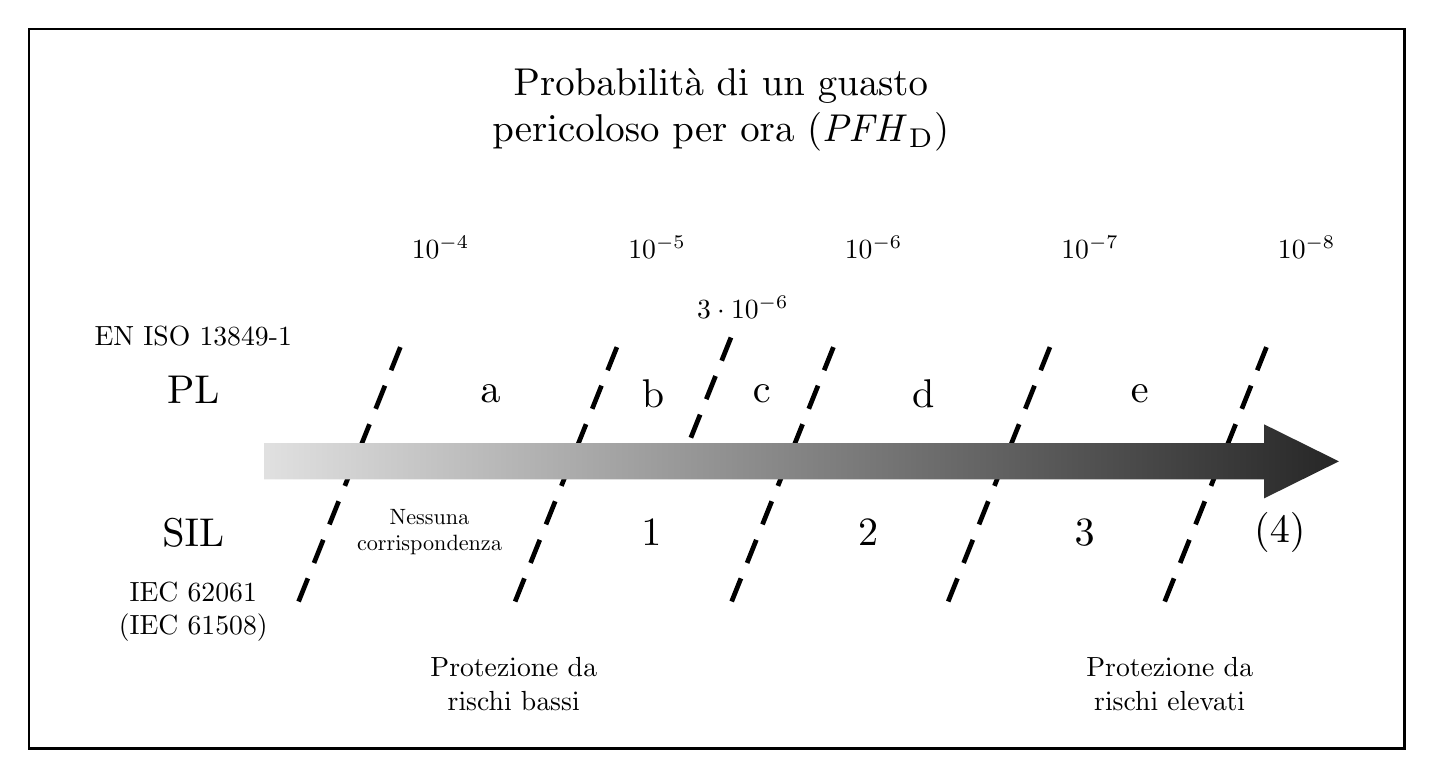
\begin{tikzpicture}[
  font=\normalsize,
  tratteggio/.style={draw=black, line width=1.7pt,
                     dash pattern=on 9pt off 6pt},
  etichetta/.style={align=center, inner sep=1pt},
  grande/.style={scale=1.45},
  piccolo/.style={scale=0.80}
]

%--------------------------------------------------------------
% Linee di separazione inclinate: una per ciascun valore di PFH_D.
% Vengono disegnate per intero e la freccia, tracciata dopo, le
% interrompe in corrispondenza della scala.
%--------------------------------------------------------------
\foreach \xpfh in {1.15, 3.90, 6.65, 9.40, 12.15}
  \draw[tratteggio] ({\xpfh-0.712},-1.78) -- ({\xpfh+0.640},1.60);
% Il limite 3*10^-6 separa PL b da PL c, ma non ha corrispondenza nei SIL
\draw[tratteggio] (5.42,0.30) -- (5.94,1.60);

%--------------------------------------------------------------
% Scala della probabilita' di guasto pericoloso per ora
%--------------------------------------------------------------
\shade[left color=black!12, right color=black!85]
  (0,-0.23) -- (12.70,-0.23) -- (12.70,-0.47) -- (13.65,0) --
  (12.70,0.47) -- (12.70,0.23) -- (0,0.23) -- cycle;

%--------------------------------------------------------------
% Titolo e valori della scala
%--------------------------------------------------------------
\node[etichetta, text width=5.7cm, scale=1.4, anchor=north] at (5.80,5.05)
  {Probabilità di un guasto\\ pericoloso per ora (\textit{PFH}\textsubscript{D})};

\node[etichetta] at (2.24,2.72)  {$10^{-4}$};
\node[etichetta] at (4.99,2.72)  {$10^{-5}$};
\node[etichetta] at (7.74,2.72)  {$10^{-6}$};
\node[etichetta] at (10.49,2.72) {$10^{-7}$};
\node[etichetta] at (13.24,2.72) {$10^{-8}$};
\node[etichetta] at (6.08,1.96)  {$3\cdot 10^{-6}$};

%--------------------------------------------------------------
% Performance Level (EN ISO 13849-1), sopra la scala
%--------------------------------------------------------------
\node[etichetta, text width=3.2cm] at (-0.90,1.59) {EN ISO 13849-1};
\node[etichetta, grande] at (-0.90,0.91) {PL};

\node[etichetta, grande] at (2.87,0.86)  {a};
\node[etichetta, grande] at (4.94,0.86)  {b};
\node[etichetta, grande] at (6.32,0.86)  {c};
\node[etichetta, grande] at (8.37,0.86)  {d};
\node[etichetta, grande] at (11.12,0.86) {e};

%--------------------------------------------------------------
% Safety Integrity Level (IEC 62061), sotto la scala
%--------------------------------------------------------------
\node[etichetta, grande] at (-0.90,-0.91) {SIL};
\node[etichetta, text width=3.2cm, anchor=north] at (-0.90,-1.50)
  {IEC 62061\\ (IEC 61508)};

\node[etichetta, text width=2.8cm, piccolo] at (2.10,-0.90)
  {Nessuna\\ corrispondenza};
\node[etichetta, grande] at (4.92,-0.90)  {1};
\node[etichetta, grande] at (7.67,-0.90)  {2};
\node[etichetta, grande] at (10.42,-0.90) {3};
\node[etichetta, grande] at (12.90,-0.90) {(4)};

%--------------------------------------------------------------
% Entita' del rischio coperto
%--------------------------------------------------------------
\node[etichetta, text width=5cm, anchor=north] at (3.17,-2.45)
  {Protezione da\\ rischi bassi};
\node[etichetta, text width=5cm, anchor=north] at (11.50,-2.45)
  {Protezione da\\ rischi elevati};

%--------------------------------------------------------------
% Cornice
%--------------------------------------------------------------
\draw[draw=black, line width=1pt]
  ([shift={(-0.45,0.45)}]current bounding box.north west) rectangle
  ([shift={(0.45,-0.45)}]current bounding box.south east);

\end{tikzpicture}
